% Annual Cognitive Science Conference
% Sample LaTeX Paper -- Proceedings Format

%% Change ``a4paper'' in the following line to ``letterpaper'' if you are
%% producing a letter-format document.

\documentclass[10pt,letterpaper]{article}
\usepackage{cogsci}
\usepackage{pslatex}
\usepackage{apacite}
\usepackage{graphicx}
\usepackage{amsmath,amsfonts}
\usepackage{tipa}
\usepackage{caption}[2005/10/24]
\newcommand{\smallspace}{\def\baselinestretch{1.1}}
\DeclareCaptionFont{smallspace}{\smallspace}
\captionsetup{
   margin    = {0pt},
   font      = {footnotesize,smallspace},
   aboveskip = {3pt},
   belowskip = {-10pt},
   labelfont = {up},
   textfont  = {up},
}

\title{Sensitivity to hypothesis sparsity in a category discrimination task}

\author{{\bf Steven Langsford} (steven.langsford@adelaide.edu.au) \\
   	{\bf Drew Hendrickson} (drew.hendrickson@adelaide.edu.au) \\
	{\bf Amy Perfors} (amy.perfors@adelaide.edu.au) \\
   	{\bf Daniel J. Navarro} (daniel.navarro@adelaide.edu.au) \\
   School of Psychology, University of Adelaide}


\begin{document}

\maketitle

\begin{abstract}
People's sensitivity to expected information value when choosing between two different types of information request was examined in a simple category-learning task. Previous work has shown that the true information value of requests can be manipulated by controlling the \textit{sparsity} of hypotheses, the degree to which category members are rare or common in the domain under consideration. However the degree to which people are sensitive to expected information value is a subject of ongoing research. This study examined a binary sorting task where sparsity differed across conditions. In contrast to previous work using visual areas to represent the coverage of a domain by a hypothesis, the stimuli in this study defined hypotheses in an abstract similarity space over geometric shapes. Participants were able to request labels for either category members or non-members. The true value of requests varied depending on the proportion of all stimuli belonging to the target category, which was known by participants. While both request types were used in all conditions, most often evenly, the proportion of participants showing a preference for one type of request was strongly impacted by the information value of that request type. A small tendency to prefer requests from the designated target category was also observed. These results are discussed in the context of previous work showing information sensitivity and positive test biases in hypothesis testing tasks.

\textbf{Keywords:} 
hypothesis testing; positive test bias; sparsity; information sensitivity;
\end{abstract}


\section*{Introduction}
Every day, countless toddlers are learning their first language by producing sentences that may or may not be grammatical, doctors are deciding which patients to refer for further testing, and novice basketball players are turning to their friends or coaches and asking ``So was \textit{that} a foul? Come on, surely that was a foul?''. Diverse as these activities are, they are all examples of hypothesis testing, and more specifically active learning, tasks where the learner has some control over what information will be recieved. The learner may be able to produce an example of a putative category for validation, as language learners do, or request a label for an opportunistically received exemplar, as in the case the unfortunate basketball player, but in either case, the question arises of how to do this efficiently \cite{settles09activelearnlitrev,gureckis2012selfdirectedlearning}. Toddlers cannot possibly test all possible combinations of words, however much they might like to, and athletes cannot challenge every play while learning the fuzzy edges of the foul rules. Exactly which examples to test though, is a non-trivial problem, and the optimal solution varies with properties of the problem domain.

So what are these good strategies, and what aspects of the problem are they sensitive to? The psychological literature has considered a number of different normative standards against which human behavior can be assessed \cite{nelson2005usefulquestions}. The traditional approach comes from the philosophy of science and treats falsificationism as the normative standard. According to this view, learners should conduct tests designed to falsify their current hypothesis, on the grounds that confirming evidence is always open to alternative explanations, but counterexamples always definitively rule out a hypothesis \cite{popper1959scidiscovery}. Strict falsification is rarely followed by people faced with hypothesis-testing tasks \cite{wason1960failure,wason1968secondlook}. Instead, a tendency to propose tests consistent with a working hypothesis has been replicated in a wide range of tasks and contexts \cite{nickerson1998confirmation}. 

Although originally considered to be an irrational bias, people's tendency to seek positive tests may have a solid statistical basis. Tests consistent with a currently preferred candidate hypothesis can falsify the hypothesis in situations where the true hypothesis is not a superset of the candidate one \cite{klayman1987confirmation}. In choosing whether to probe from within the scope of a candidate hypothesis or outside it, the learner must consider the base rate probability that a member of the domain under consideration is also a member of the target set, the proportion of domain members that are covered by the candidate hypothesis, and (estimated) positive and negative error rates under the candidate hypothesis \cite{klayman1987confirmation}. When the target set is a relatively small subset of the whole domain, and its size is approximately known, positive testing can maximize the chance of falsification of a candidate hypothesis.

Expanding on the work of \citeA{klayman1987confirmation}, recent studies have tended to assess the quality of a particular query in statistical terms. A good query might be one that minimizes the expected probability of error on a randomly selected domain member after the seeing the results of the test (expected probability gain), or returns the most information about the identity of the true hypothesis (expected information gain). Although differing in their predictions under some circumstances, these measures share the idea that a hypothesis test is a kind of gamble with uncertain rewards in terms of evidentiary value \cite{poletiek2000gambles}. Unlike strict falsification, a strategy of maximizing expected probability gain has been shown to account well for human responses in simplified hypothesis testing tasks \cite{nelson2010probgain}. 

This recent line of work opens up an important question: does people's preference for positive evidence genuinely reflect a sensitivity to its informational value, or is it a cognitive bias that just happens to produce good results in some tasks? It is this question that we consider in this paper.


\section{Hypothesis sparsity and information search}

Theoretical results showing the value of positive evidence do not imply that the positive test strategy is universally the best approach \cite{klayman1987confirmation,austerweil2011deterministic,navarro2011sparsecat}. Rather, they imply that it works when the possible hypotheses are {\it sparse}. The sparsity of a hypothesis refers to the proportion of all members of a domain that are indexed by the hypothesis in question. Sparse hypotheses index fewer than half of the members of the relevant domain \cite{navarro2011sparsecat}. For example, in the domain {\sc living species} the category {\sc dogs} is sparse, while {\sc aerobic organism} is a not sparse, since most living things are not dogs, but do metabolise oxygen. Sparsity can vary in degree: while {\sc dogs} and {\sc poodles} are both sparse categories in the domain of living things, the category {\sc poodles} is more sparse. 


Sparsity is one factor impacting the utility of the positive test strategy \cite{klayman1987confirmation, navarro2011sparsecat}. Where the target hypothesis is sparse, the expected information value of negative tests is reduced, because the probability of a negative test producing a valuable disconfirming positive result is low.
Even when the candidate hypothesis is completely misplaced, testing outside it is unlikely to land on such a small critical area, and if it is approximately correct, even this small chance is reduced. Conversely, if the target hypothesis is not sparse, the value of positive testing falls, because most positive tests return an expected and therefore uninformative positive result. This yields a natural prediction: manipulating the sparsity of the learner's hypotheses should produce a corresponding effect on the strength of the positive test bias. In fact, if hypotheses tend not to be sparse, an optimal learner should show a negative test bias. (See Figure~\ref{sparsitydemo} )

\begin{figure}[t]
\centering
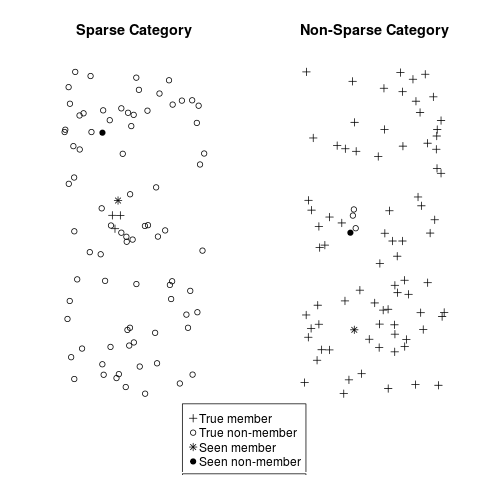
\includegraphics[width=.5\textwidth]{sparsitydemo.png}
\caption{Two simulated categories for objects varying on two dimensions. In the first case, where the category is sparse, knowing the location of a single category member is highly informative about the location of the others, and knowing the location of a single non-member is nearly totally useless. If the category is not sparse, this situation may be reversed. Positive testing is optimal when targets are both sparse and coherent.\cite{navarro2011sparsecat}}
\label{sparsitydemo}
\end{figure}

There is evidence suggesting this pattern is observed empirically. For instance,  \citeA{hendricksonInprepbattleships} had participants play a modified version of the game ``battleships''. In this task, hypotheses corresponded to a possible configuration of ships, each of which covered an area in a two dimensional space. Across experimental conditions, the size of the ships was varied, changing the sparsity of hypotheses. The predicted effect was observed: when hypotheses were not sparse, people tended to shift away from positive tests and towards negative ones. 

One potential problem with this result is that the task was highly visual, not ``conceptual'', in nature. In this case, the coverage of the possible domain by a given hypothesis was also literally the coverage of a 2D field. It is possible that the estimation of relative likelihoods apparently considered by participants was driven by an estimate of relative area particular to the visual system. In order to generalize to other active learning tasks, it must be established that the idea of coverage in a domain extends from literal physical spaces to abstract conceptual spaces. It is also possible that the extra difficulty associated with such abstract spaces makes reliance on simple heuristics such as a positive testing bias more attractive \cite{cherubini2010questionasymmetry}.

The current study aims to extend the results in \citeA{hendricksonInprepbattleships}, to see if the same effect can be observed with stimuli drawn from a more abstract stimulus space. The experiment took the form of a sorting task asking participants to learn a category boundary in a stimulus space consisting of simple geometric shapes varying on three feature-dimensions, described below. Participants were able to request labels for a randomly selected positive example of the target category or a negative non-target example. Participants were aware of what proportion of all stimuli belonged to the target category, and between-subjects manipulations of this proportion showed both a sensitivity to the information value of each type of request and a small preference for requesting positive examples.
%abstract/concrete contrast quote: `` ... recourse to asymmetric testing... probably depends on context-related motivations and prior knowledge. In abstract tasks, where that knowledge is not available, more simple strategies, such as positive testing, are prevalent'' \cite{cherubini2010questionasymmetry}

\section*{Method}
%{\bf Participants}. 

\subsection{Participants}

367 adults were recruited via Amazon Mechanical Turk.%, an online resource increasingly used and validated for experiments in psychology and linguistics \cite{sprouse11,crumpetal13}.
Of these, 301 completed the task, and 121 were excluded from further analysis for either failing to make any label requests at all (85 participants), making more than 60 requests (nine participants), or failing to sort labelled examples correctly (36 participants). Nine participants were excluded for a combination of these reasons.%so exclusions sum to 130 not 121
The remaining 180 participants contributed 360 trials, with between 104 and 131 trials falling in each of three sparsity conditions. These conditions set the proportion of stimuli belonging to the target category at 25\%, 50\%, or 75\%, hereafter { \sc sparse},{ \sc even}, and { \sc non-sparse}. Note that the only difference between the { \sc sparse} and { \sc non-sparse} conditions is one of framing, while both differ from the even condition in terms of the relative information value of requests.

Ages ranged from 19 to 67 (mean: 34.4), 45.0\% were female. 117 of the final participants were from the United States and 52 were from India. Those remaining were from eight other countries in Africa, North and South America, Europe, and Asia. All participants were paid \$0.60US for the 15 minute experiment.

\subsection{Procedure}

The cover story for the study described a fictitious company interested in harvesting a new substance called selenoid from plankton. Participants were told selenoid-rich plankton were desirable for harvesting, and were given the percentage of all plankton expected to be selenoid-rich, either 25\%, 50\%, or 75\% depending on the experimental condition. In each trial, participants were presented with two bins, each containing a random selection of half the possible plankton examples (Figure \ref{screenshot}). Buttons below each bin allowed participants to request a label for either a selenoid-rich or a selenoid-poor plankton, which appeared as a persistent coloured highlight around a randomly selected example of the requested type after a two-second delay. Plankton could be swapped between bins by clicking on them, and participants were asked to click a \textsf{submit} button after they had sorted each plankton into the correct bin.

 Once a sort was submitted, the true selenoid status for each plankton was revealed and a score displayed, calculated as 10 points for each plankton correctly sorted and -10 for each incorrectly sorted. An inference-efficiency score defined as total score divided by number of requests made was also displayed. The maximum score under this scheme was 640, the expected score due to chance zero in the {\sc even} condition and 160 in the {\sc sparse} and {\sc non-sparse} conditions. 

\begin{figure*}[t] % {figure*} ignores columns
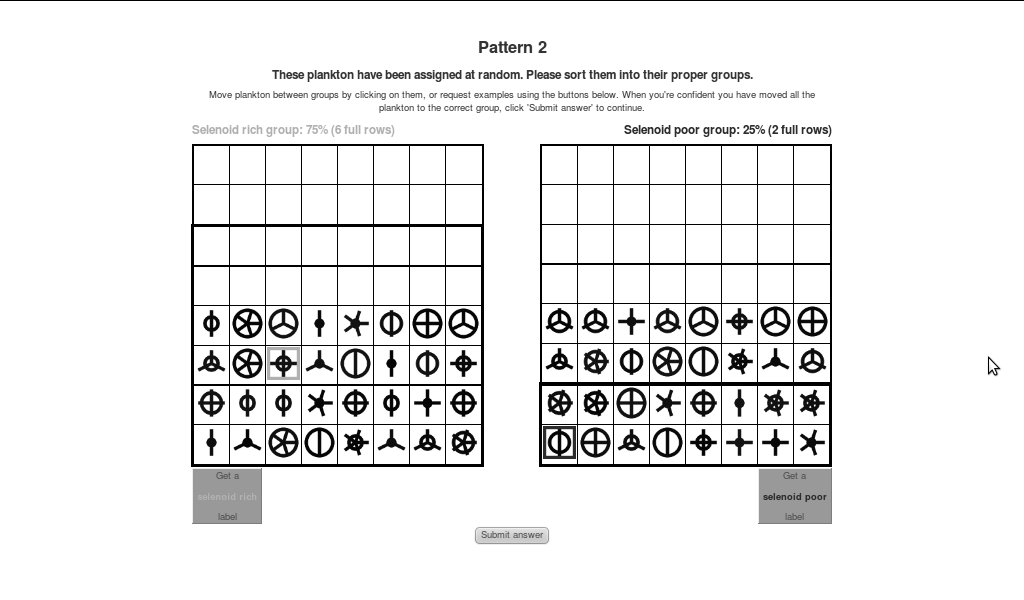
\includegraphics[width=\textwidth]{screenshot_bw.png}
\caption{Presentation of the sorting task. Information available at all times included all possible plankton examples, the proportion of plankton belonging to each group, and the request types available. Labels, if requested, appeared as a persistent coloured border around a randomly selected example of the appropriate type. An initial configuration is shown here, but two requests have been made, one of each type.}
\label{screenshot}
\end{figure*}

All participants answered a series of multiple-choice questions to make sure they had read and understood the instructions. The main task was then presented three times, the first of which was labelled as a practice trial and required participants to try all the available actions and submit a sort that respected the known proportion of plankton in each category and any visible labels. Data from this trial was not analysed. Stimuli were coloured either red, blue, or green (order randomized) across the three trials to emphasise their distinctness, with colour variation between stimuli within a single trial based on four evenly spaced points on the 255-value RGB scale for that colour.

%\subsection{Conditions}
%Meaty section in example paper... here just 25 50 75 done, best done in 'test stimuli' section?

\subsection{Stimuli}
The stimuli were geometric shapes consisting of a ring and a number of radial arms. They varied in colour intensity, size of the ring, and number of arms, with four levels in each dimension giving 64 combinations of feature values.

\begin{figure}[t]
\centering

\includegraphics[width=.3\textwidth]{minstim_bw.png}
\caption{64 different stimuli were used, corresponding to all unique combinations of four possible values on three dimensions. These were colour, ring size, and number of arms, shown here increasing from left to right.}
\end{figure}

The true selenoid status of the plankton in a given trial was determined by a threshold rule on one dimension of variation, randomly selected under the constraint that rules could not repeat across the three trials presented to any one participant. The location of this threshold was determined by sparsity condition, which varied between participants. In the {\sc sparse} and {\sc non-sparse} conditions, members of the minority group shared one extreme value on one type of feature. In the {\sc even} condition, members of the same group shared one of two adjacent values in the discriminating feature. For example, a participant in the {\sc sparse} condition might view a practice trial using red plankton in which selenoid-rich plankton had four arms and selenoid-poor plankton one, two or three, then view a trial using blue plankton where only plankton with the largest circles were rich, and finally a trial using green plankton where only the darkest shade of green were rich. Although repetition of another rule using number of arms could not have been presented to this participant after the first trial, the order of rules and whether the thresholds were high or low were completely randomized.

\section{Results}
%Did people engage with/succeed at the task?
The comparisons of interest between conditions required that participants be engaged with the task. The average score across participants was 368 of a maximum 640, corresponding to 50.4 of 64 plankton correctly sorted. Score distributions were bimodal in each condition, with one peak at the expected score due to chance (0 for {\sc even} and 160 for {\sc sparse} and {\sc non-sparse}) and the other peak at perfect performance (Figure~\ref{scorehist}).

\begin{figure}[t]
\centering
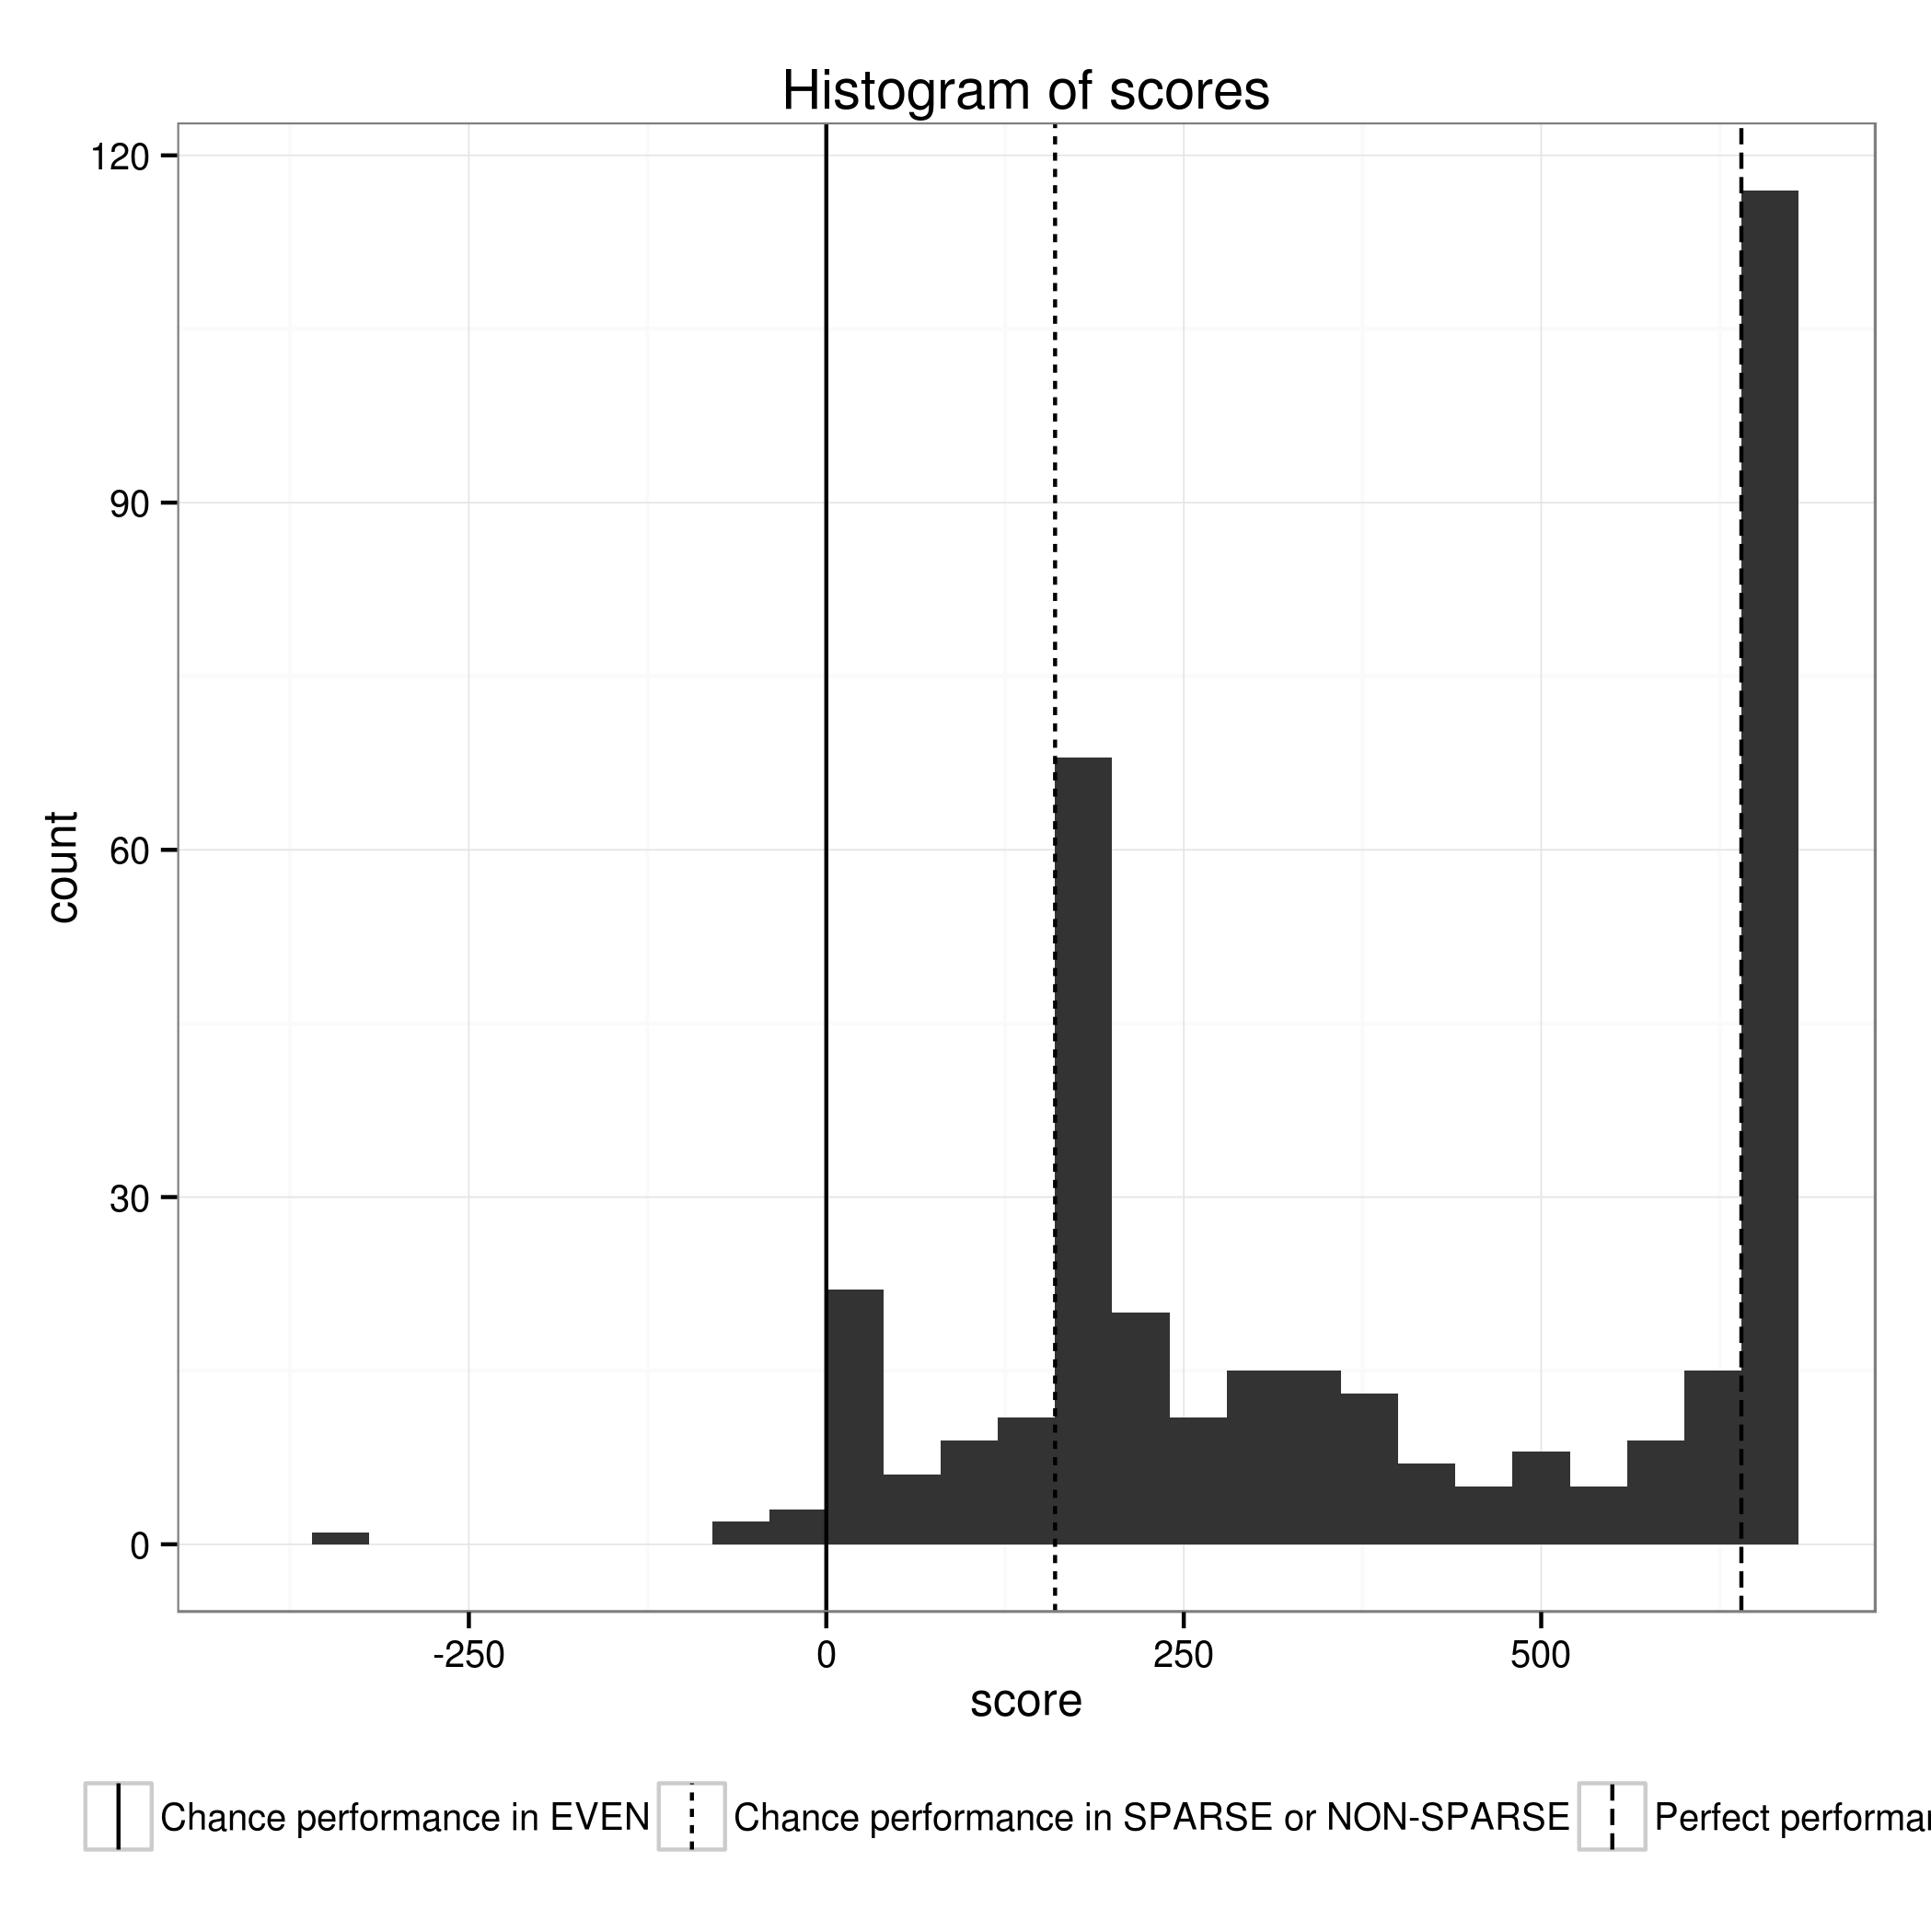
\includegraphics[width=.5\textwidth]{scoreshist.png}
\caption{The modal score in all conditions was near perfect performance, although many participants sorted with chance performance, shown as peaks in the histogram at zero in the {\sc even} condition and 160 in the {\sc sparse} and {\sc non-sparse} conditions}
\label{scorehist}
\end{figure}


While 27\% of trials scored at or below chance, many people were highly successful: on 18\% of all trials, people required fewer than six labels to sort at least 93\% correctly. The mean number of swapping actions (36.0) was close to the expected required number of swaps to correct a random sort to an ordered one (32), indicating that participants meeting the inclusion criteria above understood and engaged with the task. Scores and number of label requests were not significantly different across the first and second non-practice trials (two sample K-S test, $D=.0487, and D=.0339 respectively, p>.98$).

%(how) Were responses different in the different sparsity conditions?
Where positive testing bias predicts a preference for requests labelling the selenoid-rich plankton category regardless of the population proportions, sensitivity to the information value of requests implies a preference for requesting labels from the minority classification if this is possible. The proportion of positive requests in each trial was compared across conditions.


The proportion of positive requests differed across sparsity conditions (F(2,359) = 9.581, p<0.001, see Figure \ref{propposdots}). Specifically, the proportion of positive requests was significantly higher in the {\sc sparse} than {\sc non-sparse} (95\% HSD between .17 and .04, $p<.001$), and in {\sc even} than {\sc non-sparse}(95\% HSD between .14 and .01, $p<.02$). Potential nuisance variables trial colour, trial number, and left/right order of presentation were not found to have a significant effect (did not improve model AIC).


\begin{figure}[t]
\centering
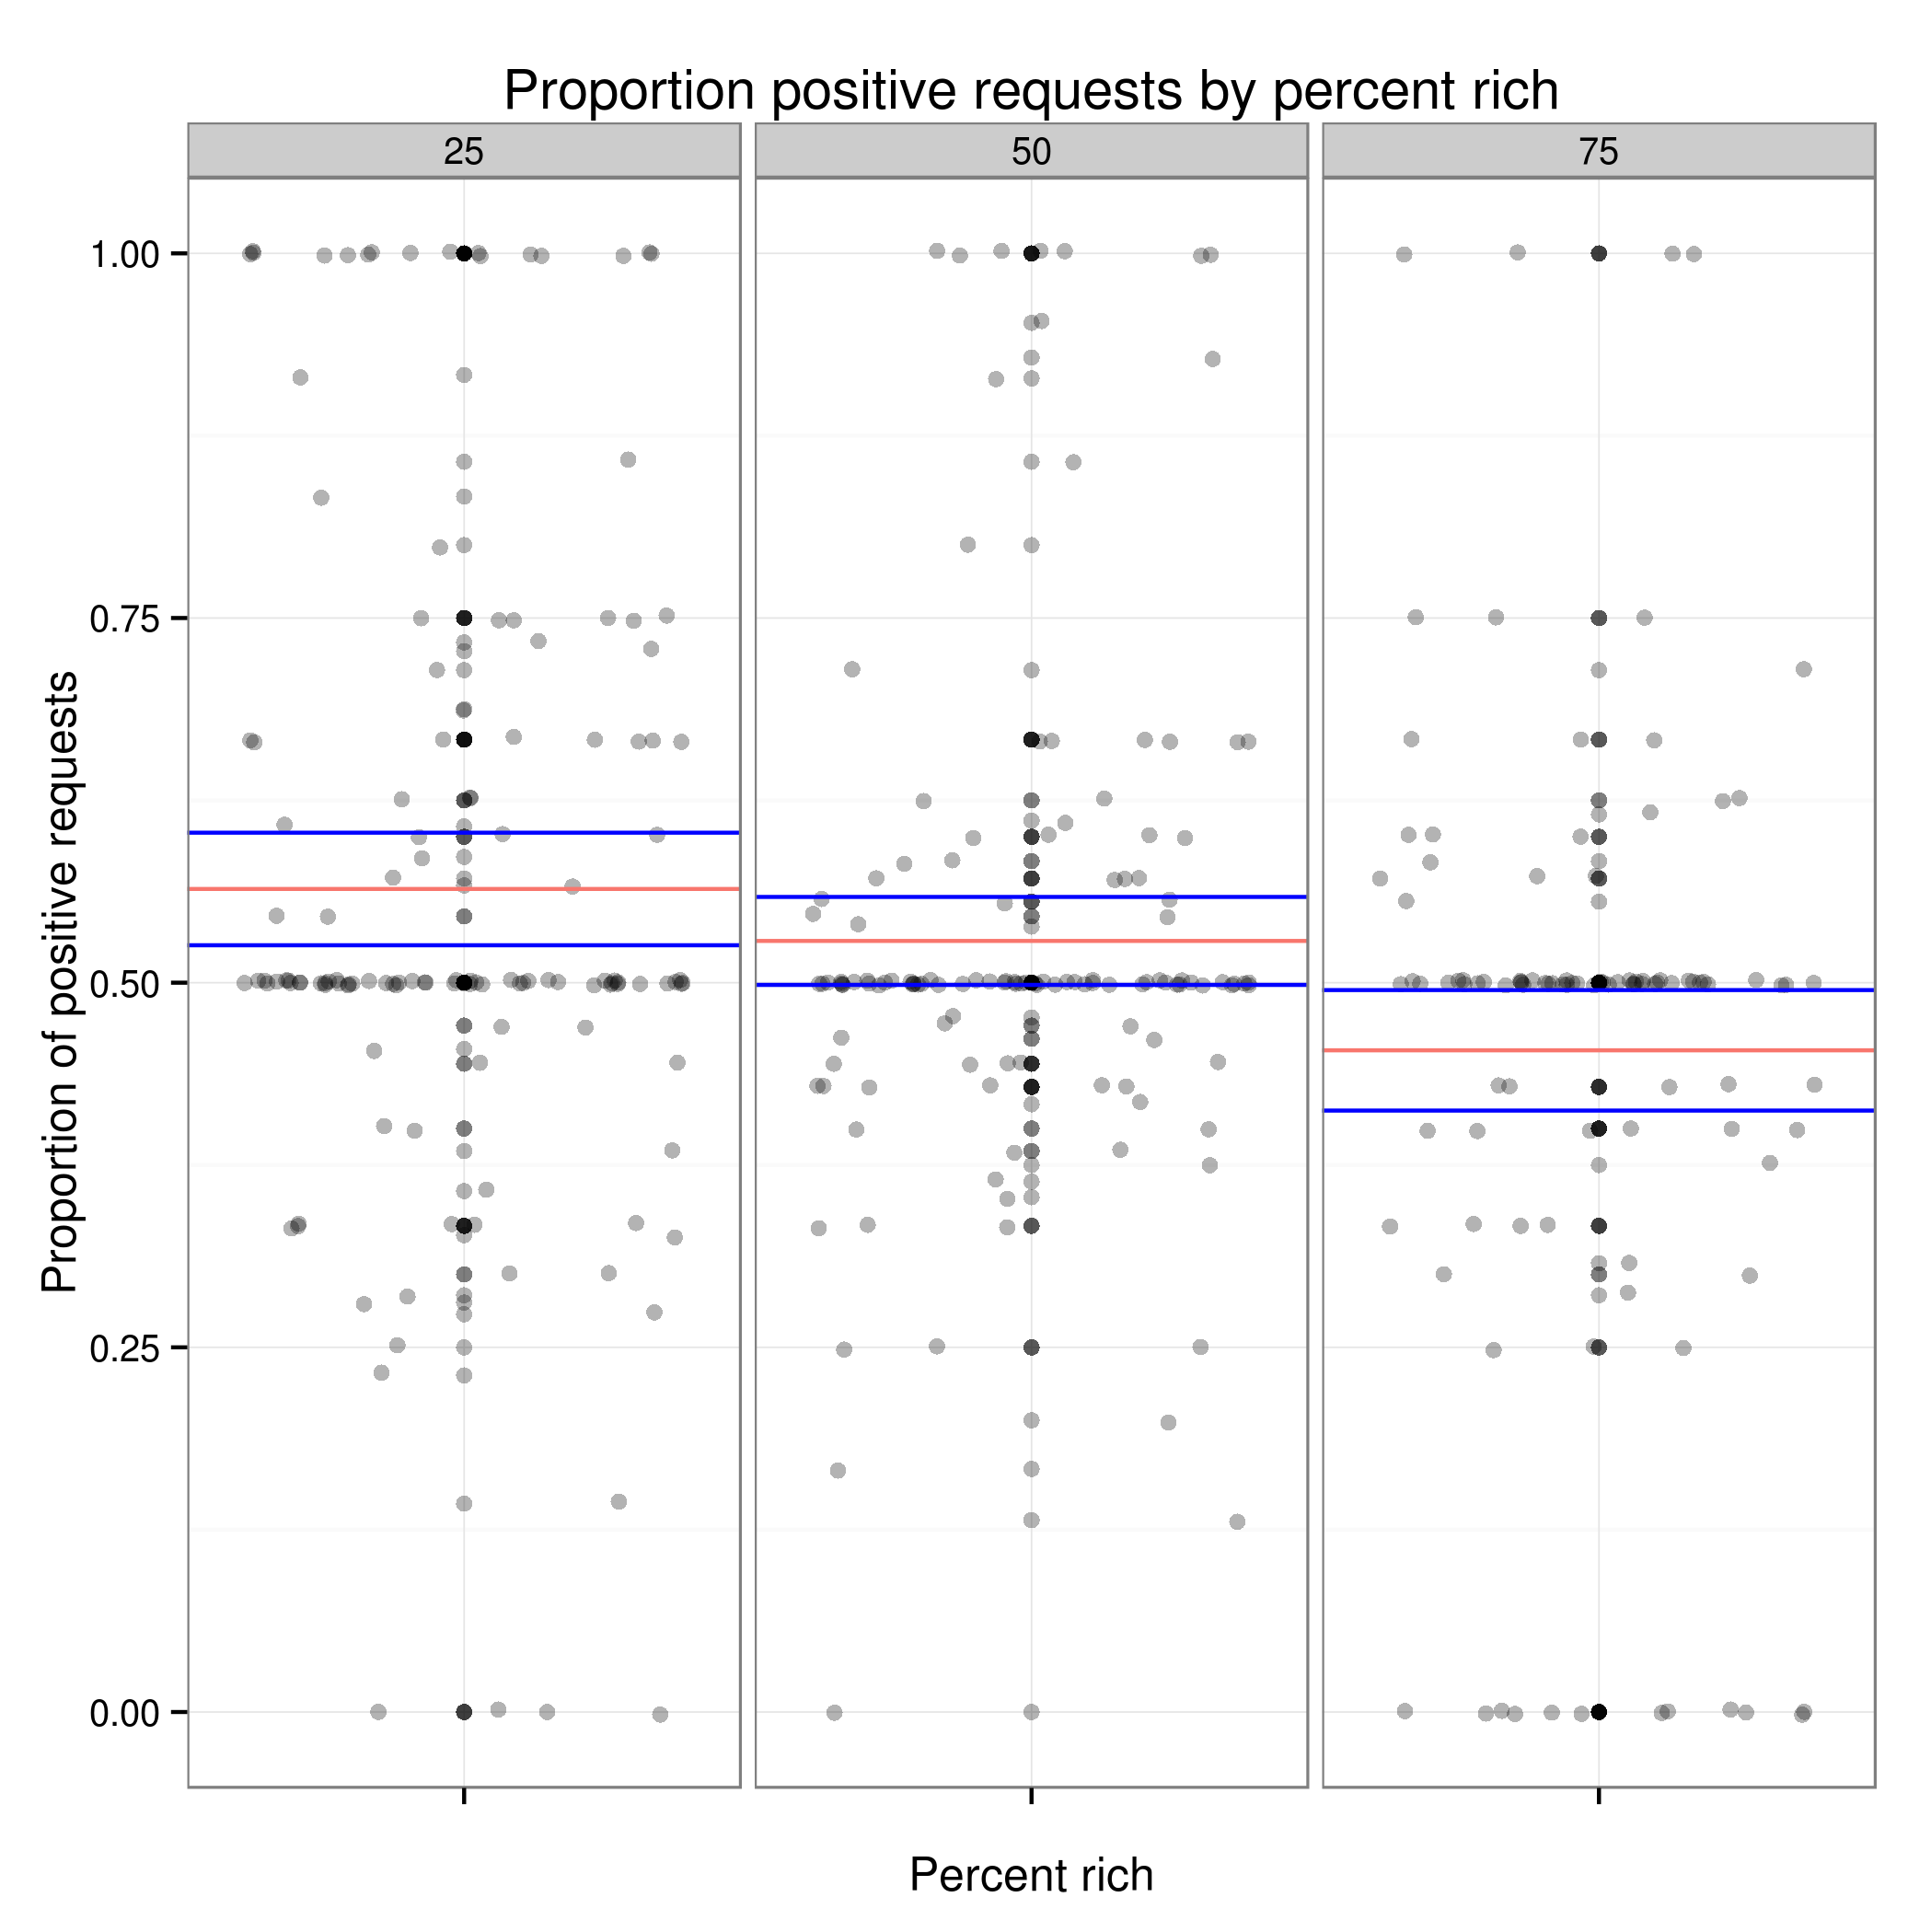
\includegraphics[width=.5\textwidth]{propposplotlines.png}
\caption{Proportion of positive requests appear to cluster at values zero, 0.5, and one. Means and 95\% confidence intervals are plotted as dark and light horizontal lines respectively. The observed differences between means may be driven by participants preferentially choosing between a small number of distinct request strategies.}
\label{propposdots}
\end{figure}

As Figure \ref{propposdots} shows, the differences in means do not appear to reflect a large-scale shift in requests for all individuals from condition to condition. Rather, in all conditions, responses tended to cluster at the special values of one (all positive), zero (all negative), and 0.5 (even). The proportion of people choosing each strategy is what appears to shift between conditions. We can test whether this is truly occurring by categorizing responses by request strategy, as in Figure \ref{sidebysidebar3}. An \textit{even} request strategy was defined as a proportion of positive requests falling between 0.45 and 0.55, with \textit{Prefers positive} and \textit{Prefers negative} responses falling above and below these values (Figure~\ref{sidebysidebar3}).

\begin{figure}[t]
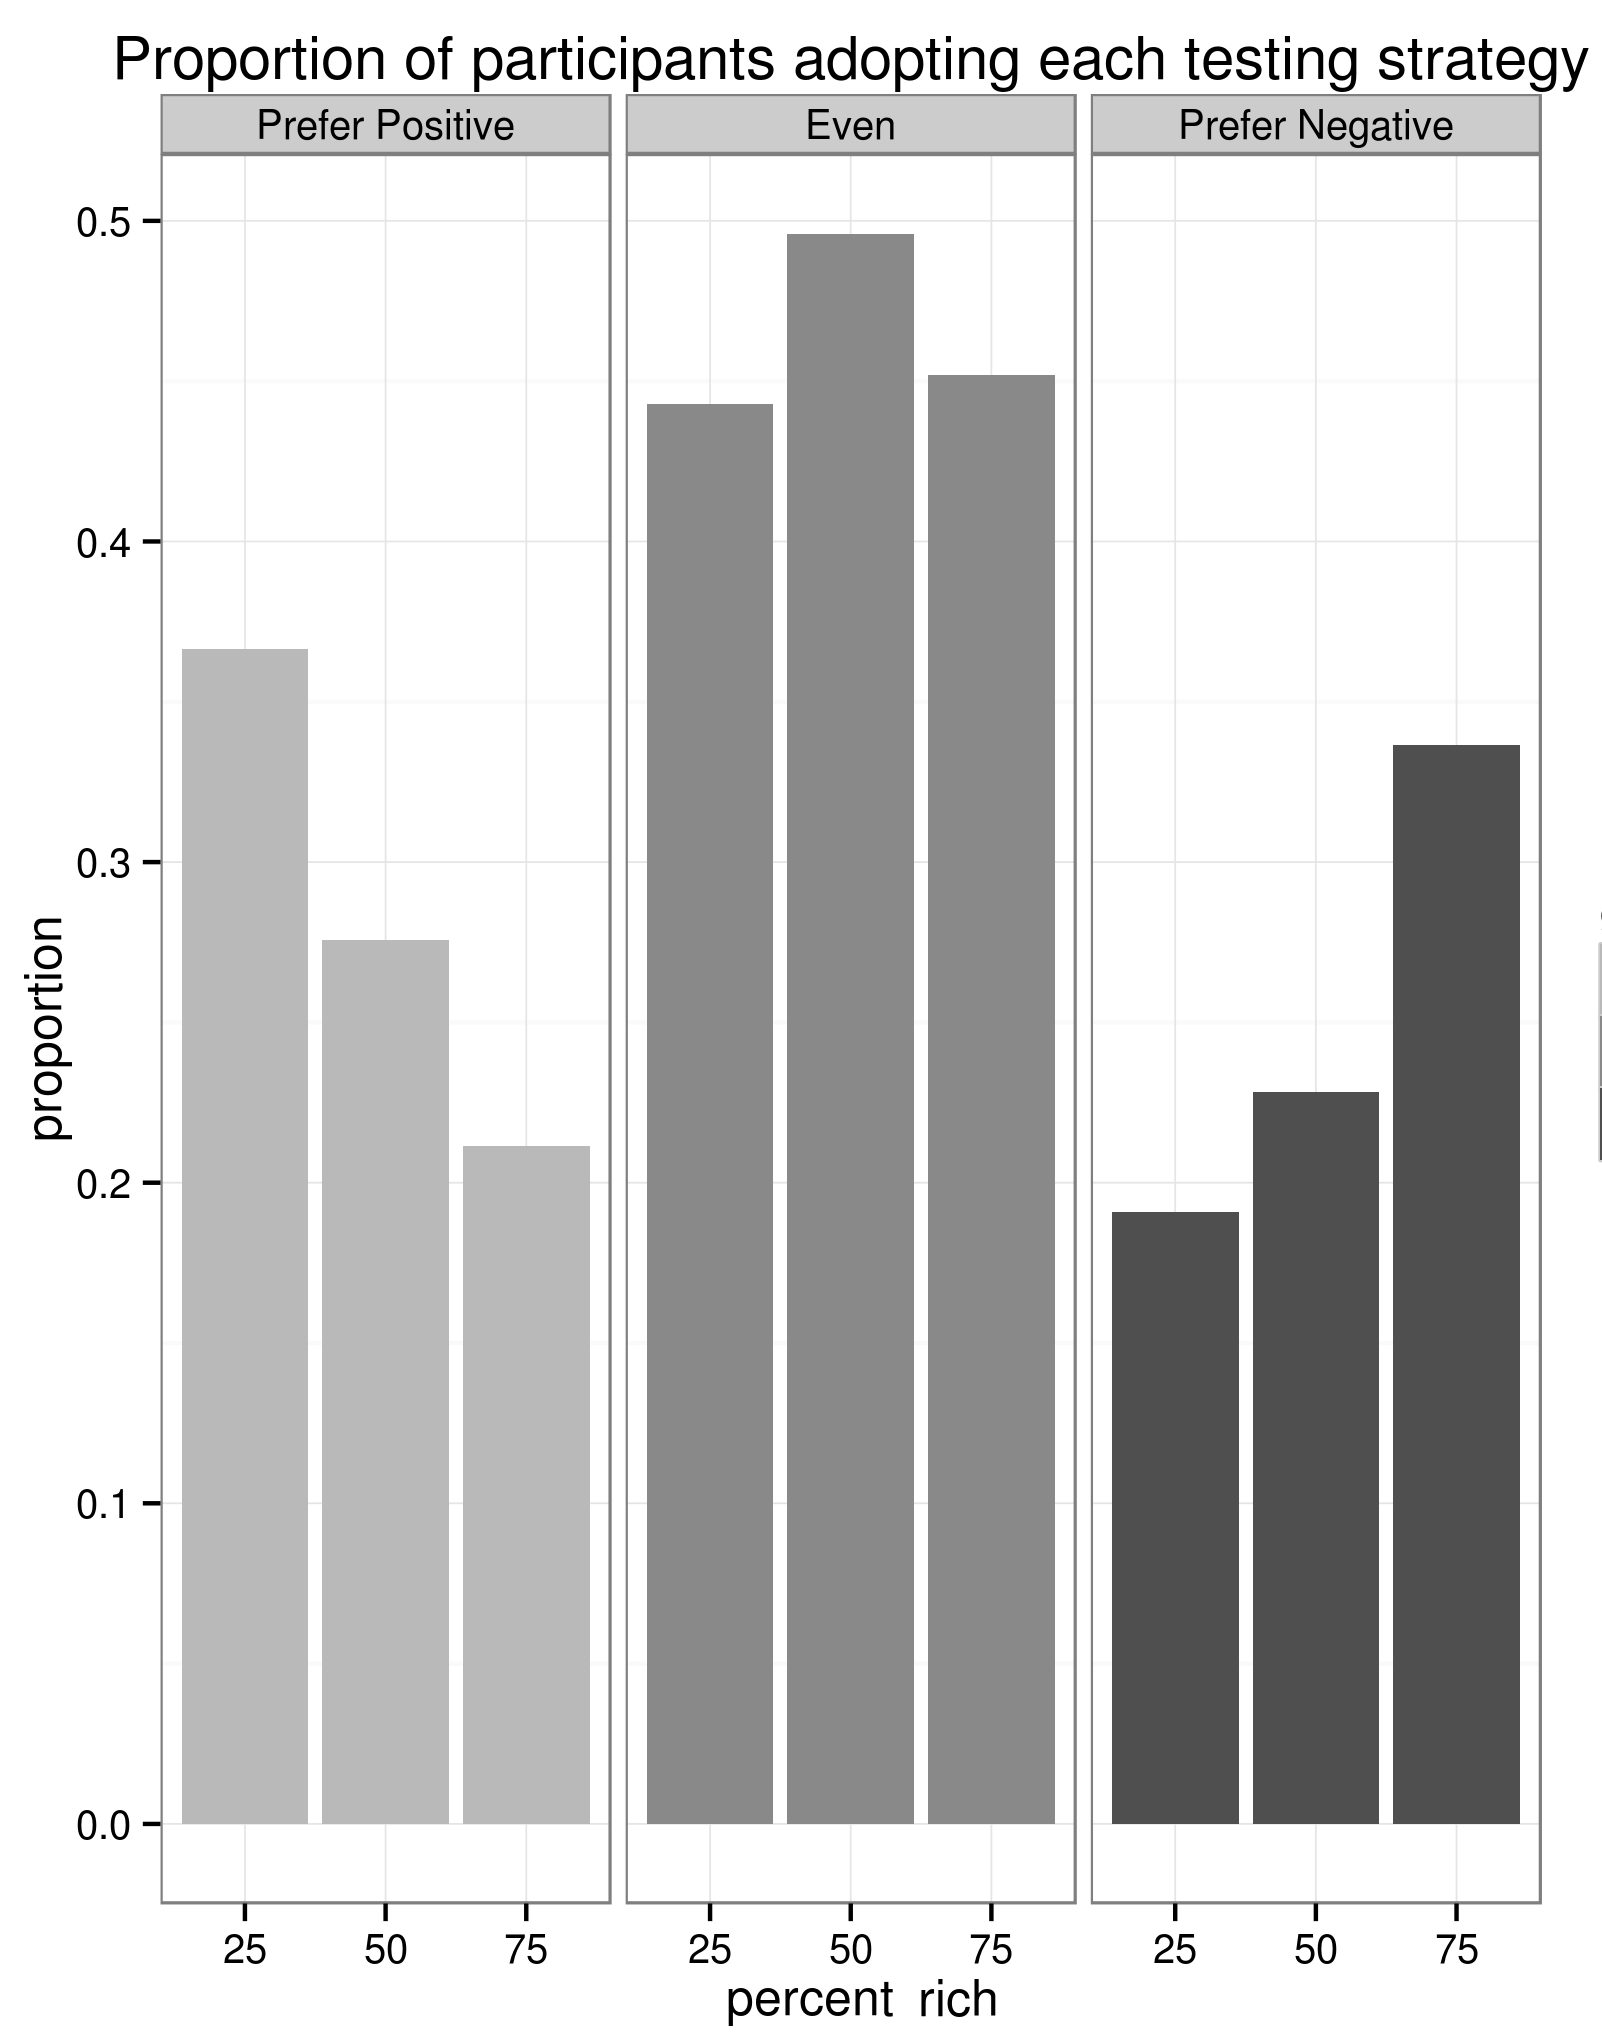
\includegraphics[width=.5\textwidth]{sidebysidebar3_nolegendbw.png}
\caption{Proportion of participants using each testing strategy in the three conditions. Requesting equal amounts of information from both possible categorizations was popular in all conditions, however when population proportions were unequal, a greater proportion of participants began to prefer requests from the minority group. This preference was somewhat asymmetrical, with people more readily switching to preferring positive requests}
\label{sidebysidebar3}
\end{figure}

All strategies were followed by some participants in all conditions, but the proportion of participants selecting each strategy differed significantly between conditions ($\chi^2_2=13.16,p<.01$). %chisq.text(table(actiondat$actiontype,actiondat$percentrich)[c(2,4),]) #is this the right test?
The \textit{even} request strategy balancing positive and negative requests was always most popular, however the proportion of people preferring positive tests was higher in the {\sc sparse} condition than in the {\sc non-sparse} condition. The inverse pattern was observed for negative tests, indicating a preference for whichever type of test corresponded to the minority classification in the whole population. Such a preference is consistent with the greater information value of minority requests. As Figure \ref{sidebysidebar3} shows, this preference is evident even when the minority group is framed as a negative non-target group.

Since the only difference between the {\sc sparse} and {\sc non-sparse} conditions is one of framing, if request choice is driven by expected information gain, request preferences should be simply reversed between these two conditions. Figure \ref{sidebysidebar3} shows a slight asymmetry whereby positive preferential strategies are more often chosen. Collapsing across conditions, .48 of all information requests recorded in this study were for selenoid-poor labels (1192 of 2482 total requests), and .52 were for selenoid-rich labels (1290 of 2482 total requests), a small but significant difference in favour of positive requests despite the symmetry of the task structure $(\chi^2_1=7.74, p<.01)$. %Right test stat? From: prop.test(c(1192,1290),c(2482,2482))

To examine whether participant's apparent sensitivity to sparsity was in fact driven by a subset of participants, trials were partitioned by score into high-scoring `solved' trials (score over 600, n=117), and lower-scoring trials (score less than or equal to 600, n=245). Both high-scoring trials and low-scoring trials showed the same clustering pattern at zero,.5,and one, with .5 the most popular strategy. Both show an increased tendency to switch to preferring labels of the minority categorization, although this pattern is significant only in the higher scoring group ($F=13.04$, $p<.01$) and not significant in the lower-scoring group ($F=1.63$, $p>.1$)(Figure \ref{dotsbyscore}).

\begin{figure}[t]
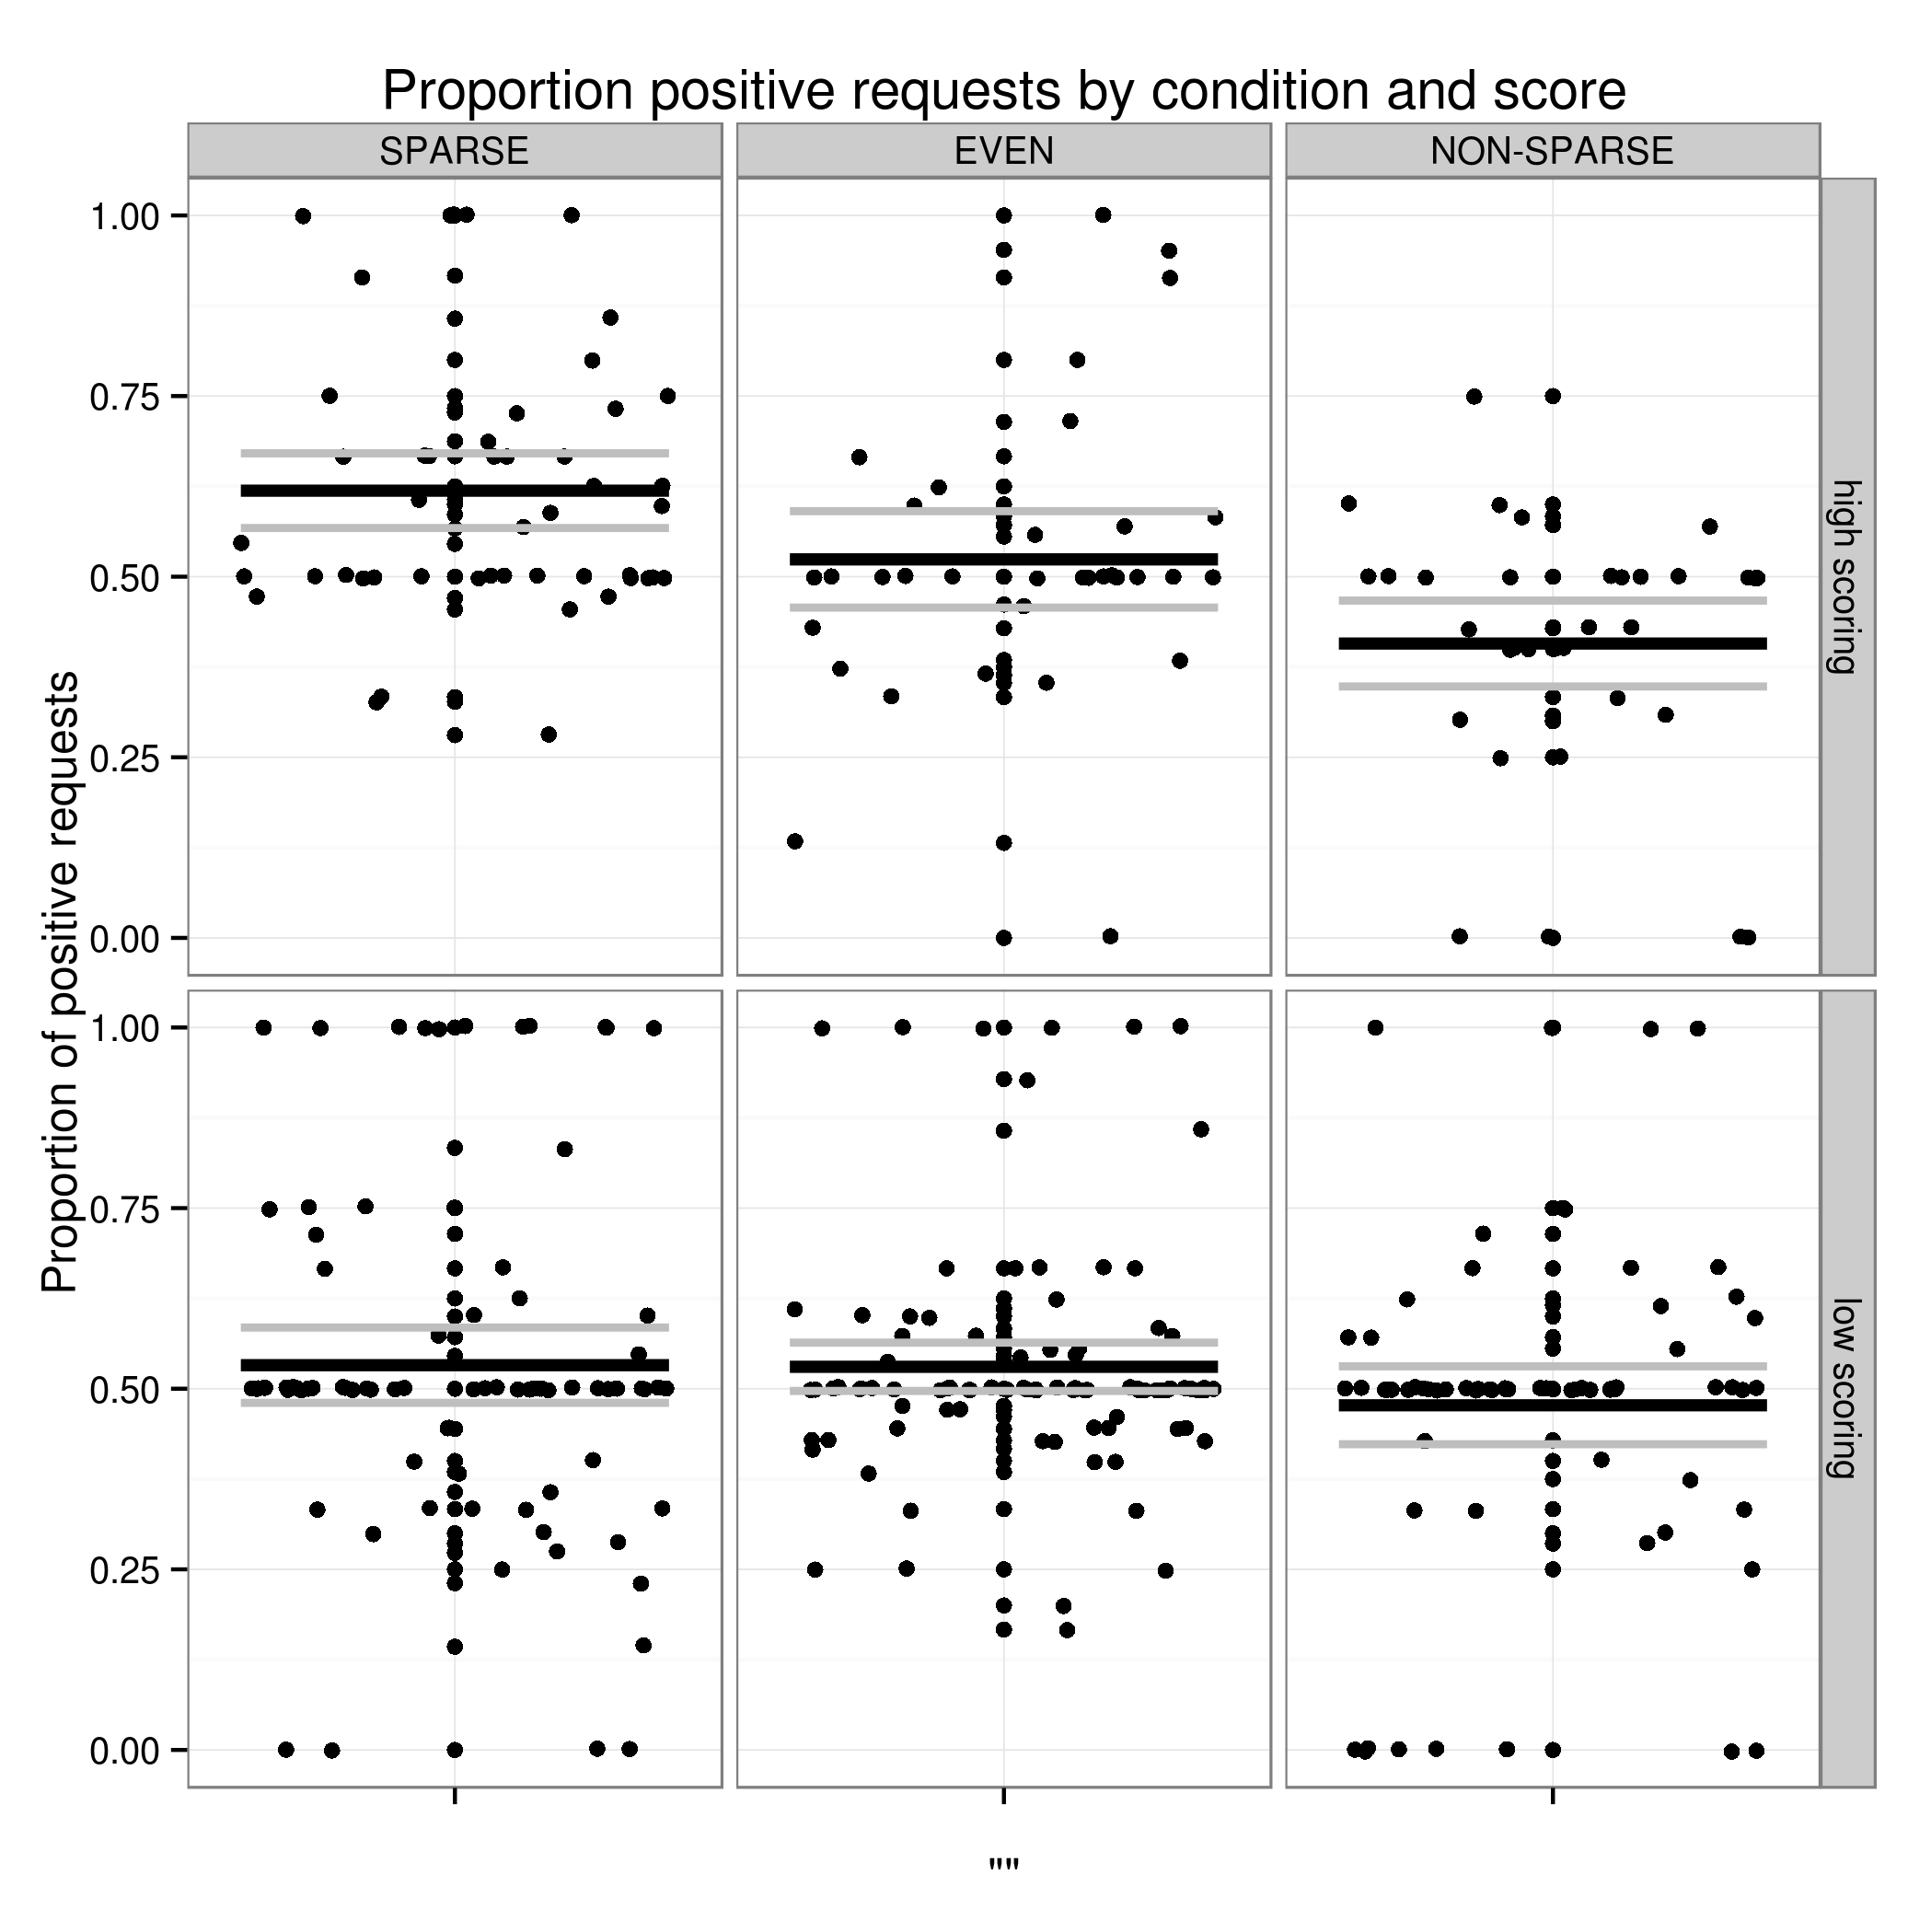
\includegraphics[width=.5\textwidth]{dotsbyscore.png}
\caption{Differences in mean proportion positive requests significant in the higher scoring group, and not significant, although in the same direction, in the lower scoring group.}
\label{dotsbyscore}
\end{figure}

\section{Discussion}
%Conclusions
The results show people adjusting their sampling strategies in response to the sparsity of the hypothesis testing task at hand, supporting an information sensitive account of natural hypothesis testing\cite{navarro2011sparsecat}. This sensitivity to the relative size of the target category in the stimulus space obtains even though this is an abstract space defined over the similarity of a set of geometrical shapes. The observed behavour is inconsistent with a strong bias towards positive testing, which predicts a difference between the symmetrical {\sc sparse} and {\sc non-sparse} conditions due to the change of frame. No strong difference was observed, although positive tests were more popular than negative tests overall. 

Individual participants reflected sensitivity to the information value of the different request types in a coarse-grained way, gravitating to either balanced requests or requests of a single type. The \textit{even} strategy was always most popular, regardless of condition. This may reflect a popular explorative heuristic that motiviates people to use all available request types, or possibly simply a lack of engagement with the task.This second alternative is somewhat supported by the observation that preferential strategies were used more among the highest scoring participants. Despite the popularity of the \textit{even} strategy, the attractiveness of the uneven preferential strategies scaled as predicted with changes in the true information value of requests. For this to be the case, the value of requests must have been estimated (not necessarily explicitly) by participants from information available about category sparsity. Such information is often available or can be estimated in real-world category learning tasks, even when the universe of all possible examples is large, for example by estimating a base rate probability from an observed frequency, or through more sophisticated capture-recapture estimation techniques %\cite{pollock1990capturerecapture}
(also not necessarily explicit) when repeatedly encountering novel and familiar examples of a category.%hmm, where is that types-vs-tokens sampling discussion?
The behaviour observed in the context of the plankton-sorting task suggests that to the extent that category sparsity information is available, it could be expected to impact the perceived attractiveness of different types of information request, ie. preferences for positive or negative testing.

Although consistent with a degree of sensitivity to the information value of requests, these data show a number of ways in which people's requests deviate from information-utility treatments of the task. 

Some positive testing bias is suggested, with participants favouring the target rich category asymmetrically despite the symmetry of the sparsity manipulation. It is unclear if this is due to a form of matching \cite{evans1998matching} on the target most prominent in the instructions, or an expectation that the conditions that favour positive testing are generally ubiquitous, although in this artificial case they are not.

The clustering of positive-test proportions at the special values zero, .5, and one in all conditions also suggests a kind of heuristic approach, albeit a heuristic that is to some extent context sensitive. It is unclear from these results if this clustering is reflective of granularity in the perception of information utility, granularity in responding after accurate perception of request utility, or simply an artifact of the fact that participants were limited to two different request types, which to some extent naturally emphasises these values, especially for small numbers of requests.

%Limitations
 A number of features of the presentation are also open to question. All possible plankton shapes were visible to participants at all times, a situation unlikely with natural categories, but one which might influence the use of sparsity information, since estimating the proportion of stimuli indexed by a hypothesis in a given domain requires an estimate of the boundaries of that domain. Similarly, the density of examples was even across the stimulus space, with one example of each kind of plankton, a condition which need not hold in general. The true category rules were also highly restricted, in that they were all thresholds on a single dimension, binary, and strictly complementary. Natural categories are often non-binary, nested or otherwise overlapping, and often involve multiple dimensions. 

Further work is required to explore how people weigh up the value of information-seeking actions under these more complex conditions. The results presented here suggest that some such consideration of information utility is an essential component of any complete description of natural active concept learning. Where hypothesis sparsity information is available, as it is in many natural domains, people's information-seeking behaviour is informed by the structure of the domain, even when that structure is abstract and conceptual in nature.

%Missed one: visual box around plankton undermines claim of abstract space? Other holes...?

\section{Acknowledgements}

This research was supported by... 

\renewcommand{\bibliographytypesize}{\footnotesize}
\bibliographystyle{apacite}

\setlength{\bibleftmargin}{.125in}
\setlength{\bibindent}{-\bibleftmargin}


\bibliography{plankton.bib}


\end{document}
